\documentclass{standalone}
\usepackage{tikz}
\usetikzlibrary{patterns, positioning}


\begin{document}
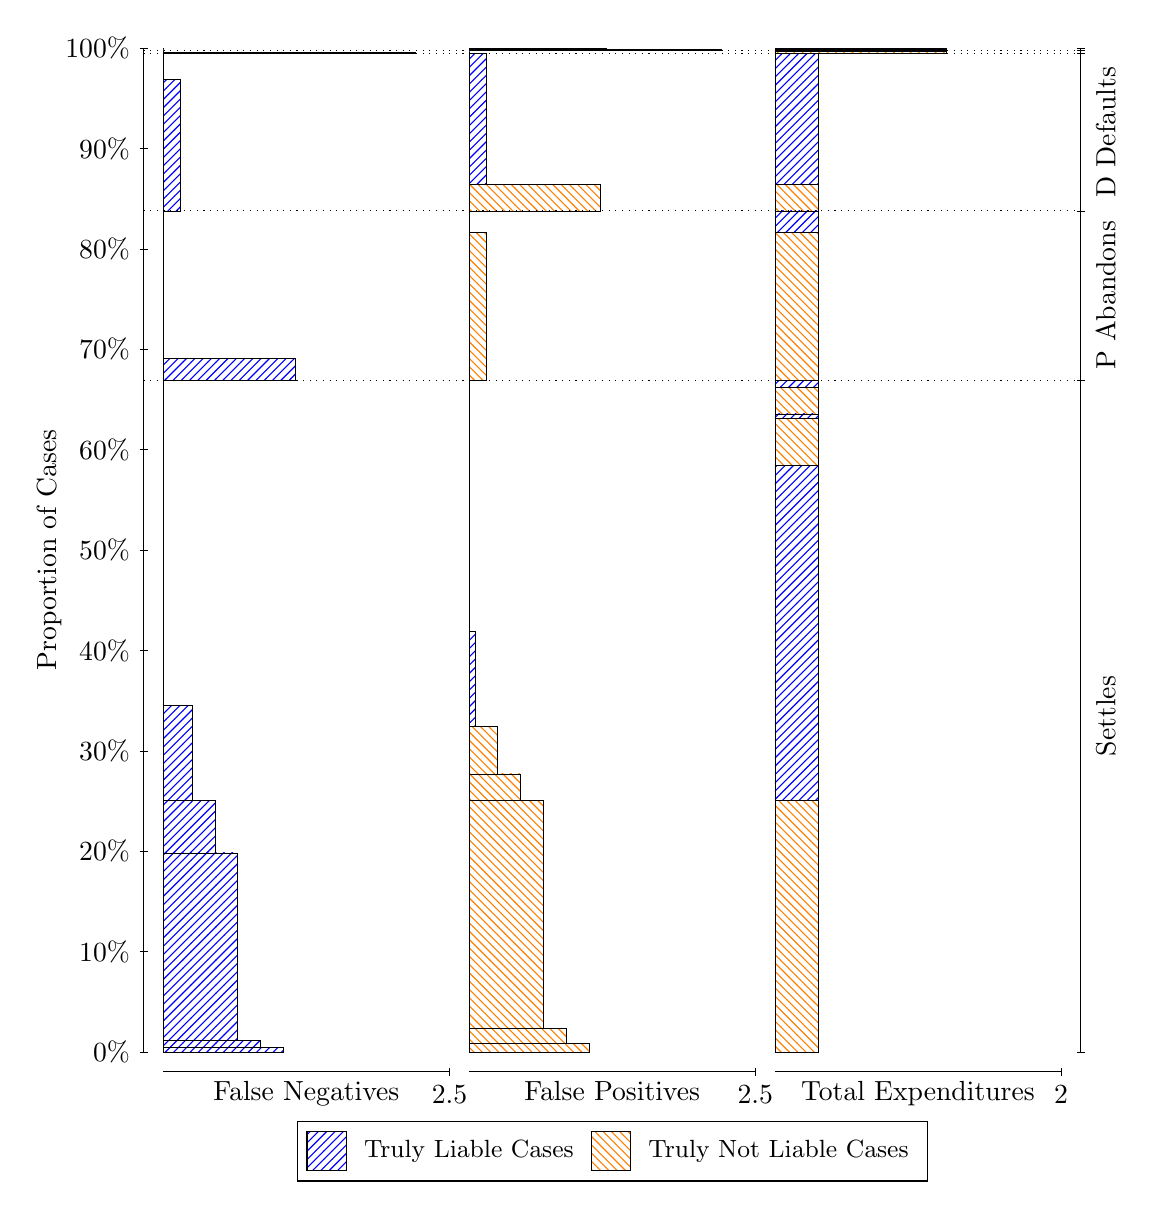
\begin{tikzpicture}
\draw[black, very thin] (1.5,1.75) -- (1.5,14.5);
\node[rotate=90, text=black, anchor=center] at (0.3, 8.125) {Proportion of Cases};
\draw[black, very thin] (1.45,1.75) -- (1.55,1.75);
\node[text=black, anchor=east] at (1.45, 1.75) {0\%};
\draw[black, very thin] (1.45,3.025) -- (1.55,3.025);
\node[text=black, anchor=east] at (1.45, 3.025) {10\%};
\draw[black, very thin] (1.45,4.3) -- (1.55,4.3);
\node[text=black, anchor=east] at (1.45, 4.3) {20\%};
\draw[black, very thin] (1.45,5.575) -- (1.55,5.575);
\node[text=black, anchor=east] at (1.45, 5.575) {30\%};
\draw[black, very thin] (1.45,6.85) -- (1.55,6.85);
\node[text=black, anchor=east] at (1.45, 6.85) {40\%};
\draw[black, very thin] (1.45,8.125) -- (1.55,8.125);
\node[text=black, anchor=east] at (1.45, 8.125) {50\%};
\draw[black, very thin] (1.45,9.4) -- (1.55,9.4);
\node[text=black, anchor=east] at (1.45, 9.4) {60\%};
\draw[black, very thin] (1.45,10.675) -- (1.55,10.675);
\node[text=black, anchor=east] at (1.45, 10.675) {70\%};
\draw[black, very thin] (1.45,11.95) -- (1.55,11.95);
\node[text=black, anchor=east] at (1.45, 11.95) {80\%};
\draw[black, very thin] (1.45,13.225) -- (1.55,13.225);
\node[text=black, anchor=east] at (1.45, 13.225) {90\%};
\draw[black, very thin] (1.45,14.5) -- (1.55,14.5);
\node[text=black, anchor=east] at (1.45, 14.5) {100\%};

\draw[black, very thin] (13.4,1.75) -- (13.4,14.5);
\draw[black, very thin] (13.35,1.75) -- (13.45,1.75);
\node[anchor=west] at (13.35, 1.75) {};
\draw[black, very thin] (13.35,10.283) -- (13.45,10.283);
\node[anchor=west] at (13.35, 10.283) {};
\draw[black, very thin] (13.35,12.433) -- (13.45,12.433);
\node[anchor=west] at (13.35, 12.433) {};
\draw[black, very thin] (13.35,14.431) -- (13.45,14.431);
\node[anchor=west] at (13.35, 14.431) {};
\draw[black, very thin] (13.35,14.469) -- (13.45,14.469);
\node[anchor=west] at (13.35, 14.469) {};
\draw[black, very thin] (13.35,14.5) -- (13.45,14.5);
\node[anchor=west] at (13.35, 14.5) {};

\draw[black, very thin, pattern color=blue, pattern=north east lines] (1.75,1.75) rectangle (3.276,1.8064);
\draw[black, very thin, pattern color=blue, pattern=north east lines] (1.75,1.8064) rectangle (2.9853,1.9015);
\draw[black, very thin, pattern color=blue, pattern=north east lines] (1.75,1.9015) rectangle (2.6947,4.2785);
\draw[black, very thin, pattern color=blue, pattern=north east lines] (1.75,4.2785) rectangle (2.404,4.9459);
\draw[black, very thin, pattern color=blue, pattern=north east lines] (1.75,4.9459) rectangle (2.1133,6.1496);
\draw[black, very thin, pattern color=orange, pattern=north west lines] (1.75,6.1496) rectangle (1.75,10.283);
\draw[black, very thin, pattern color=blue, pattern=north east lines] (1.75,10.283) rectangle (3.4213,10.561);
\draw[black, very thin, pattern color=orange, pattern=north west lines] (1.75,10.561) rectangle (1.75,12.433);
\draw[black, very thin, pattern color=blue, pattern=north east lines] (1.75,12.433) rectangle (1.968,14.099);
\draw[black, very thin, pattern color=orange, pattern=north west lines] (1.75,14.099) rectangle (1.75,14.431);
\draw[black, very thin, pattern color=blue, pattern=north east lines] (1.75,14.431) rectangle (4.9473,14.442);
\draw[black, very thin, pattern color=orange, pattern=north west lines] (1.75,14.442) rectangle (1.75,14.469);
\draw[black, very thin, pattern color=orange, pattern=north west lines] (1.75,14.469) rectangle (1.75,14.48);
\draw[black, very thin, pattern color=blue, pattern=north east lines] (1.75,14.48) rectangle (1.75,14.5);
\draw[black, very thin, pattern color=orange, pattern=north west lines] (5.6333,1.75) rectangle (7.1593,1.8629);
\draw[black, very thin, pattern color=orange, pattern=north west lines] (5.6333,1.8629) rectangle (6.8687,2.0532);
\draw[black, very thin, pattern color=orange, pattern=north west lines] (5.6333,2.0532) rectangle (6.578,4.9478);
\draw[black, very thin, pattern color=orange, pattern=north west lines] (5.6333,4.9478) rectangle (6.2873,5.2815);
\draw[black, very thin, pattern color=orange, pattern=north west lines] (5.6333,5.2815) rectangle (5.9967,5.883);
\draw[black, very thin, pattern color=blue, pattern=north east lines] (5.6333,5.883) rectangle (5.706,7.0868);
\draw[black, very thin, pattern color=blue, pattern=north east lines] (5.6333,7.0868) rectangle (5.6333,10.283);
\draw[black, very thin, pattern color=orange, pattern=north west lines] (5.6333,10.283) rectangle (5.8513,12.155);
\draw[black, very thin, pattern color=blue, pattern=north east lines] (5.6333,12.155) rectangle (5.6333,12.433);
\draw[black, very thin, pattern color=orange, pattern=north west lines] (5.6333,12.433) rectangle (7.3047,12.765);
\draw[black, very thin, pattern color=blue, pattern=north east lines] (5.6333,12.765) rectangle (5.8513,14.431);
\draw[black, very thin, pattern color=orange, pattern=north west lines] (5.6333,14.431) rectangle (5.6333,14.457);
\draw[black, very thin, pattern color=blue, pattern=north east lines] (5.6333,14.457) rectangle (5.6333,14.469);
\draw[black, very thin, pattern color=orange, pattern=north west lines] (5.6333,14.469) rectangle (8.8307,14.48);
\draw[black, very thin, pattern color=blue, pattern=north east lines] (5.6333,14.48) rectangle (7.3773,14.5);
\draw[black, very thin, pattern color=orange, pattern=north west lines] (9.5167,1.75) rectangle (10.062,4.9478);
\draw[black, very thin, pattern color=blue, pattern=north east lines] (9.5167,4.9478) rectangle (10.062,9.196);
\draw[black, very thin, pattern color=orange, pattern=north west lines] (9.5167,9.196) rectangle (10.062,9.7976);
\draw[black, very thin, pattern color=blue, pattern=north east lines] (9.5167,9.7976) rectangle (10.062,9.854);
\draw[black, very thin, pattern color=orange, pattern=north west lines] (9.5167,9.854) rectangle (10.062,10.188);
\draw[black, very thin, pattern color=blue, pattern=north east lines] (9.5167,10.188) rectangle (10.062,10.283);
\draw[black, very thin, pattern color=orange, pattern=north west lines] (9.5167,10.283) rectangle (10.062,12.155);
\draw[black, very thin, pattern color=blue, pattern=north east lines] (9.5167,12.155) rectangle (10.062,12.433);
\draw[black, very thin, pattern color=orange, pattern=north west lines] (9.5167,12.433) rectangle (10.062,12.765);
\draw[black, very thin, pattern color=blue, pattern=north east lines] (9.5167,12.765) rectangle (10.062,14.431);
\draw[black, very thin, pattern color=orange, pattern=north west lines] (9.5167,14.431) rectangle (11.697,14.457);
\draw[black, very thin, pattern color=blue, pattern=north east lines] (9.5167,14.457) rectangle (11.697,14.469);
\draw[black, very thin, pattern color=orange, pattern=north west lines] (9.5167,14.469) rectangle (11.697,14.48);
\draw[black, very thin, pattern color=blue, pattern=north east lines] (9.5167,14.48) rectangle (11.697,14.5);
\draw[black, dotted] (1.5,10.283) -- (13.4,10.283);
\draw[black, dotted] (1.5,12.433) -- (13.4,12.433);
\draw[black, dotted] (1.5,14.431) -- (13.4,14.431);
\draw[black, dotted] (1.5,14.469) -- (13.4,14.469);
\draw[black, very thin] (1.75,1.5) -- (5.3833,1.5);
\node[text=black, anchor=north] at (3.5667, 1.5) {False Negatives};
\draw[black, very thin] (5.3833,1.45) -- (5.3833,1.55);
\node[text=black, anchor=north] at (5.3833, 1.45) {2.5};

\draw[black, very thin] (5.6333,1.5) -- (9.2667,1.5);
\node[text=black, anchor=north] at (7.45, 1.5) {False Positives};
\draw[black, very thin] (9.2667,1.45) -- (9.2667,1.55);
\node[text=black, anchor=north] at (9.2667, 1.45) {2.5};

\draw[black, very thin] (9.5167,1.5) -- (13.15,1.5);
\node[text=black, anchor=north] at (11.333, 1.5) {Total Expenditures};
\draw[black, very thin] (13.15,1.45) -- (13.15,1.55);
\node[text=black, anchor=north] at (13.15, 1.45) {2};

\node[text=black, centered, rotate=90] at (13.72, 6.0163) {Settles};
\node[text=black, centered, rotate=90] at (13.72, 11.358) {P Abandons};
\node[text=black, centered, rotate=90] at (13.72, 13.432) {D Defaults};



\draw (7.449999999999999,1.5) node[draw=none] (baseCoordinate) {};
\begin{scope}[align=center]
        \matrix[scale=0.5, draw=black, below=0.5cm of baseCoordinate, nodes={draw}, column sep=0.1cm]{
            \node[rectangle, draw, minimum width=0.5cm, minimum height=0.5cm, pattern color=blue, pattern=north east lines] {}; &
            \node[draw=none, font=\small, text=black] (B) {Truly Liable Cases}; &
            \node[rectangle, draw, minimum width=0.5cm, minimum height=0.5cm, pattern color=orange, pattern=north west lines] {}; &
            \node[draw=none, font=\small, text=black] (B) {Truly Not Liable Cases}; \\
            };
\end{scope}

\end{tikzpicture}
\end{document}